% Options for packages loaded elsewhere
\PassOptionsToPackage{unicode}{hyperref}
\PassOptionsToPackage{hyphens}{url}
\PassOptionsToPackage{dvipsnames,svgnames,x11names}{xcolor}
%
\documentclass[
  letterpaper,
  DIV=11,
  numbers=noendperiod]{scrreprt}

\usepackage{amsmath,amssymb}
\usepackage{iftex}
\ifPDFTeX
  \usepackage[T1]{fontenc}
  \usepackage[utf8]{inputenc}
  \usepackage{textcomp} % provide euro and other symbols
\else % if luatex or xetex
  \usepackage{unicode-math}
  \defaultfontfeatures{Scale=MatchLowercase}
  \defaultfontfeatures[\rmfamily]{Ligatures=TeX,Scale=1}
\fi
\usepackage{lmodern}
\ifPDFTeX\else  
    % xetex/luatex font selection
\fi
% Use upquote if available, for straight quotes in verbatim environments
\IfFileExists{upquote.sty}{\usepackage{upquote}}{}
\IfFileExists{microtype.sty}{% use microtype if available
  \usepackage[]{microtype}
  \UseMicrotypeSet[protrusion]{basicmath} % disable protrusion for tt fonts
}{}
\makeatletter
\@ifundefined{KOMAClassName}{% if non-KOMA class
  \IfFileExists{parskip.sty}{%
    \usepackage{parskip}
  }{% else
    \setlength{\parindent}{0pt}
    \setlength{\parskip}{6pt plus 2pt minus 1pt}}
}{% if KOMA class
  \KOMAoptions{parskip=half}}
\makeatother
\usepackage{xcolor}
\setlength{\emergencystretch}{3em} % prevent overfull lines
\setcounter{secnumdepth}{5}
% Make \paragraph and \subparagraph free-standing
\ifx\paragraph\undefined\else
  \let\oldparagraph\paragraph
  \renewcommand{\paragraph}[1]{\oldparagraph{#1}\mbox{}}
\fi
\ifx\subparagraph\undefined\else
  \let\oldsubparagraph\subparagraph
  \renewcommand{\subparagraph}[1]{\oldsubparagraph{#1}\mbox{}}
\fi

\usepackage{color}
\usepackage{fancyvrb}
\newcommand{\VerbBar}{|}
\newcommand{\VERB}{\Verb[commandchars=\\\{\}]}
\DefineVerbatimEnvironment{Highlighting}{Verbatim}{commandchars=\\\{\}}
% Add ',fontsize=\small' for more characters per line
\usepackage{framed}
\definecolor{shadecolor}{RGB}{241,243,245}
\newenvironment{Shaded}{\begin{snugshade}}{\end{snugshade}}
\newcommand{\AlertTok}[1]{\textcolor[rgb]{0.68,0.00,0.00}{#1}}
\newcommand{\AnnotationTok}[1]{\textcolor[rgb]{0.37,0.37,0.37}{#1}}
\newcommand{\AttributeTok}[1]{\textcolor[rgb]{0.40,0.45,0.13}{#1}}
\newcommand{\BaseNTok}[1]{\textcolor[rgb]{0.68,0.00,0.00}{#1}}
\newcommand{\BuiltInTok}[1]{\textcolor[rgb]{0.00,0.23,0.31}{#1}}
\newcommand{\CharTok}[1]{\textcolor[rgb]{0.13,0.47,0.30}{#1}}
\newcommand{\CommentTok}[1]{\textcolor[rgb]{0.37,0.37,0.37}{#1}}
\newcommand{\CommentVarTok}[1]{\textcolor[rgb]{0.37,0.37,0.37}{\textit{#1}}}
\newcommand{\ConstantTok}[1]{\textcolor[rgb]{0.56,0.35,0.01}{#1}}
\newcommand{\ControlFlowTok}[1]{\textcolor[rgb]{0.00,0.23,0.31}{#1}}
\newcommand{\DataTypeTok}[1]{\textcolor[rgb]{0.68,0.00,0.00}{#1}}
\newcommand{\DecValTok}[1]{\textcolor[rgb]{0.68,0.00,0.00}{#1}}
\newcommand{\DocumentationTok}[1]{\textcolor[rgb]{0.37,0.37,0.37}{\textit{#1}}}
\newcommand{\ErrorTok}[1]{\textcolor[rgb]{0.68,0.00,0.00}{#1}}
\newcommand{\ExtensionTok}[1]{\textcolor[rgb]{0.00,0.23,0.31}{#1}}
\newcommand{\FloatTok}[1]{\textcolor[rgb]{0.68,0.00,0.00}{#1}}
\newcommand{\FunctionTok}[1]{\textcolor[rgb]{0.28,0.35,0.67}{#1}}
\newcommand{\ImportTok}[1]{\textcolor[rgb]{0.00,0.46,0.62}{#1}}
\newcommand{\InformationTok}[1]{\textcolor[rgb]{0.37,0.37,0.37}{#1}}
\newcommand{\KeywordTok}[1]{\textcolor[rgb]{0.00,0.23,0.31}{#1}}
\newcommand{\NormalTok}[1]{\textcolor[rgb]{0.00,0.23,0.31}{#1}}
\newcommand{\OperatorTok}[1]{\textcolor[rgb]{0.37,0.37,0.37}{#1}}
\newcommand{\OtherTok}[1]{\textcolor[rgb]{0.00,0.23,0.31}{#1}}
\newcommand{\PreprocessorTok}[1]{\textcolor[rgb]{0.68,0.00,0.00}{#1}}
\newcommand{\RegionMarkerTok}[1]{\textcolor[rgb]{0.00,0.23,0.31}{#1}}
\newcommand{\SpecialCharTok}[1]{\textcolor[rgb]{0.37,0.37,0.37}{#1}}
\newcommand{\SpecialStringTok}[1]{\textcolor[rgb]{0.13,0.47,0.30}{#1}}
\newcommand{\StringTok}[1]{\textcolor[rgb]{0.13,0.47,0.30}{#1}}
\newcommand{\VariableTok}[1]{\textcolor[rgb]{0.07,0.07,0.07}{#1}}
\newcommand{\VerbatimStringTok}[1]{\textcolor[rgb]{0.13,0.47,0.30}{#1}}
\newcommand{\WarningTok}[1]{\textcolor[rgb]{0.37,0.37,0.37}{\textit{#1}}}

\providecommand{\tightlist}{%
  \setlength{\itemsep}{0pt}\setlength{\parskip}{0pt}}\usepackage{longtable,booktabs,array}
\usepackage{calc} % for calculating minipage widths
% Correct order of tables after \paragraph or \subparagraph
\usepackage{etoolbox}
\makeatletter
\patchcmd\longtable{\par}{\if@noskipsec\mbox{}\fi\par}{}{}
\makeatother
% Allow footnotes in longtable head/foot
\IfFileExists{footnotehyper.sty}{\usepackage{footnotehyper}}{\usepackage{footnote}}
\makesavenoteenv{longtable}
\usepackage{graphicx}
\makeatletter
\def\maxwidth{\ifdim\Gin@nat@width>\linewidth\linewidth\else\Gin@nat@width\fi}
\def\maxheight{\ifdim\Gin@nat@height>\textheight\textheight\else\Gin@nat@height\fi}
\makeatother
% Scale images if necessary, so that they will not overflow the page
% margins by default, and it is still possible to overwrite the defaults
% using explicit options in \includegraphics[width, height, ...]{}
\setkeys{Gin}{width=\maxwidth,height=\maxheight,keepaspectratio}
% Set default figure placement to htbp
\makeatletter
\def\fps@figure{htbp}
\makeatother

\KOMAoption{captions}{tableheading}
\makeatletter
\@ifpackageloaded{tcolorbox}{}{\usepackage[skins,breakable]{tcolorbox}}
\@ifpackageloaded{fontawesome5}{}{\usepackage{fontawesome5}}
\definecolor{quarto-callout-color}{HTML}{909090}
\definecolor{quarto-callout-note-color}{HTML}{0758E5}
\definecolor{quarto-callout-important-color}{HTML}{CC1914}
\definecolor{quarto-callout-warning-color}{HTML}{EB9113}
\definecolor{quarto-callout-tip-color}{HTML}{00A047}
\definecolor{quarto-callout-caution-color}{HTML}{FC5300}
\definecolor{quarto-callout-color-frame}{HTML}{acacac}
\definecolor{quarto-callout-note-color-frame}{HTML}{4582ec}
\definecolor{quarto-callout-important-color-frame}{HTML}{d9534f}
\definecolor{quarto-callout-warning-color-frame}{HTML}{f0ad4e}
\definecolor{quarto-callout-tip-color-frame}{HTML}{02b875}
\definecolor{quarto-callout-caution-color-frame}{HTML}{fd7e14}
\makeatother
\makeatletter
\makeatother
\makeatletter
\@ifpackageloaded{bookmark}{}{\usepackage{bookmark}}
\makeatother
\makeatletter
\@ifpackageloaded{caption}{}{\usepackage{caption}}
\AtBeginDocument{%
\ifdefined\contentsname
  \renewcommand*\contentsname{Table of contents}
\else
  \newcommand\contentsname{Table of contents}
\fi
\ifdefined\listfigurename
  \renewcommand*\listfigurename{List of Figures}
\else
  \newcommand\listfigurename{List of Figures}
\fi
\ifdefined\listtablename
  \renewcommand*\listtablename{List of Tables}
\else
  \newcommand\listtablename{List of Tables}
\fi
\ifdefined\figurename
  \renewcommand*\figurename{Figure}
\else
  \newcommand\figurename{Figure}
\fi
\ifdefined\tablename
  \renewcommand*\tablename{Table}
\else
  \newcommand\tablename{Table}
\fi
}
\@ifpackageloaded{float}{}{\usepackage{float}}
\floatstyle{ruled}
\@ifundefined{c@chapter}{\newfloat{codelisting}{h}{lop}}{\newfloat{codelisting}{h}{lop}[chapter]}
\floatname{codelisting}{Listing}
\newcommand*\listoflistings{\listof{codelisting}{List of Listings}}
\makeatother
\makeatletter
\@ifpackageloaded{caption}{}{\usepackage{caption}}
\@ifpackageloaded{subcaption}{}{\usepackage{subcaption}}
\makeatother
\makeatletter
\@ifpackageloaded{tcolorbox}{}{\usepackage[skins,breakable]{tcolorbox}}
\makeatother
\makeatletter
\@ifundefined{shadecolor}{\definecolor{shadecolor}{rgb}{.97, .97, .97}}
\makeatother
\makeatletter
\makeatother
\makeatletter
\makeatother
\ifLuaTeX
  \usepackage{selnolig}  % disable illegal ligatures
\fi
\IfFileExists{bookmark.sty}{\usepackage{bookmark}}{\usepackage{hyperref}}
\IfFileExists{xurl.sty}{\usepackage{xurl}}{} % add URL line breaks if available
\urlstyle{same} % disable monospaced font for URLs
\hypersetup{
  pdftitle={recTiles},
  pdfauthor={Julia Schedler},
  colorlinks=true,
  linkcolor={blue},
  filecolor={Maroon},
  citecolor={Blue},
  urlcolor={Blue},
  pdfcreator={LaTeX via pandoc}}

\title{recTiles}
\author{Julia Schedler}
\date{2023-07-10}

\begin{document}
\maketitle
\ifdefined\Shaded\renewenvironment{Shaded}{\begin{tcolorbox}[sharp corners, enhanced, interior hidden, boxrule=0pt, breakable, borderline west={3pt}{0pt}{shadecolor}, frame hidden]}{\end{tcolorbox}}\fi

\renewcommand*\contentsname{Table of contents}
{
\hypersetup{linkcolor=}
\setcounter{tocdepth}{2}
\tableofcontents
}
\bookmarksetup{startatroot}

\hypertarget{tiles}{%
\chapter*{Tiles}\label{tiles}}
\addcontentsline{toc}{chapter}{Tiles}

\markboth{Tiles}{Tiles}

This is Julia's transcription of what Alex has been showing her so far
about his tile stuff.

\bookmarksetup{startatroot}

\hypertarget{julias-first-tiles}{%
\chapter*{Julia's First Tiles}\label{julias-first-tiles}}
\addcontentsline{toc}{chapter}{Julia's First Tiles}

\markboth{Julia's First Tiles}{Julia's First Tiles}

\hypertarget{hand-drawn}{%
\section*{Hand-drawn}\label{hand-drawn}}
\addcontentsline{toc}{section}{Hand-drawn}

\markright{Hand-drawn}

\hypertarget{first-tile}{%
\subsection*{First Tile}\label{first-tile}}
\addcontentsline{toc}{subsection}{First Tile}

\begin{figure}

{\centering \includegraphics{images/first_by_hand.png}

}

\caption{Actually I did this one second, but this is the first matrix I
chose. Alex suggested I change to the one visualized next.}

\end{figure}

\[
M = \begin{bmatrix}2 & 1\\ -1 & 1\end{bmatrix}
\]

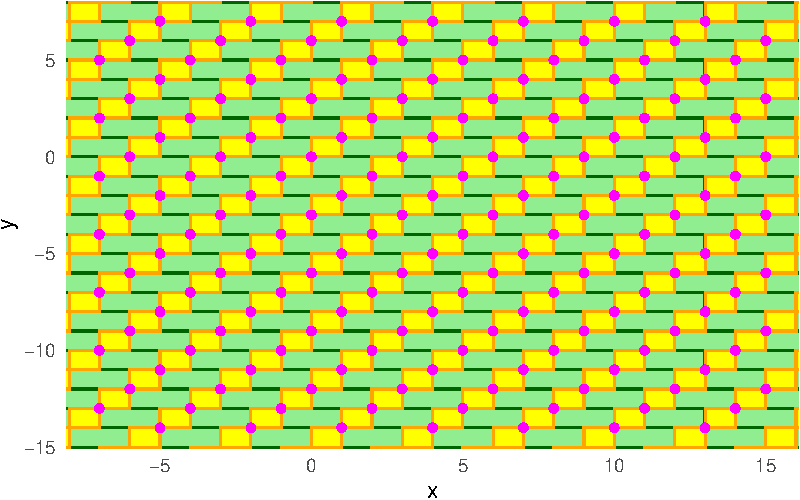
\includegraphics{handdrawn_files/figure-pdf/first-1.pdf}

\hypertarget{second-tile}{%
\subsection*{Second Tile}\label{second-tile}}
\addcontentsline{toc}{subsection}{Second Tile}

\begin{figure}

{\centering \includegraphics{images/second_by_hand.png}

}

\caption{The second tiling, actually the very first that I drew (well,
the first I drew correctly-\/- see my mistake?)}

\end{figure}

\[
M = \begin{bmatrix} 2 & 5\\ -1 & 3\end{bmatrix}
\]

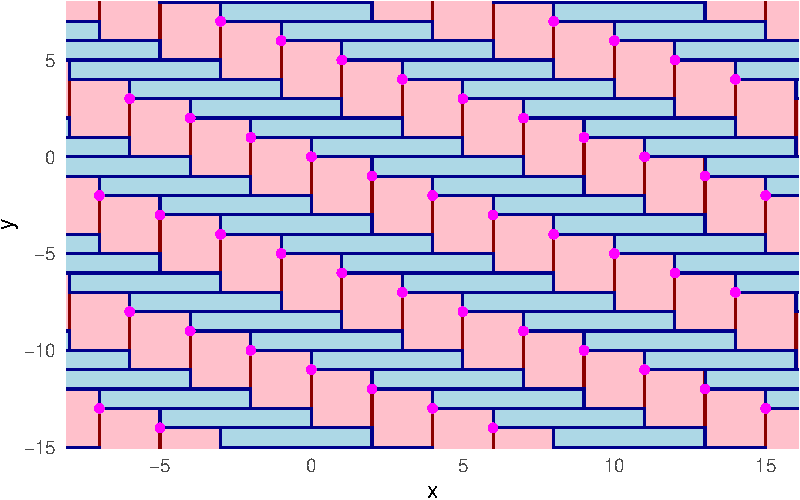
\includegraphics{handdrawn_files/figure-pdf/second-1.pdf}

\hypertarget{third-tile}{%
\subsection*{Third Tile}\label{third-tile}}
\addcontentsline{toc}{subsection}{Third Tile}

\begin{figure}

{\centering \includegraphics{images/third_by_hand.png}

}

\caption{The drawing for the third tiling. I did this one for fun by
myself! I chose big numbers so I could have space to write out
coordinates and work out some math for the purposes of coding it up.}

\end{figure}

\[
M = \begin{bmatrix} 8& 5\\ -4 & 3\end{bmatrix}
\]

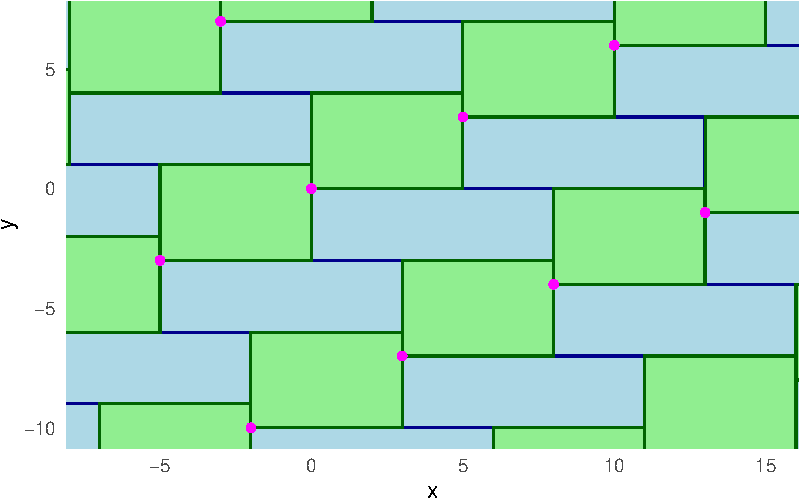
\includegraphics{handdrawn_files/figure-pdf/third-1.pdf}

\hypertarget{computer-generated}{%
\section*{Computer-generated}\label{computer-generated}}
\addcontentsline{toc}{section}{Computer-generated}

\markright{Computer-generated}

\hypertarget{fourth-tile}{%
\subsection*{Fourth Tile}\label{fourth-tile}}
\addcontentsline{toc}{subsection}{Fourth Tile}

\[
M = \begin{bmatrix} 3 & 3\\ -3 & 3\end{bmatrix}
\]

\begin{Shaded}
\begin{Highlighting}[]
\FunctionTok{library}\NormalTok{(ggplot2)}
\DocumentationTok{\#\# original coordinates}
\NormalTok{A }\OtherTok{\textless{}{-}} \FunctionTok{matrix}\NormalTok{(}\FunctionTok{c}\NormalTok{(}\DecValTok{3}\NormalTok{, }\SpecialCharTok{{-}}\DecValTok{3}\NormalTok{), }\AttributeTok{ncol =} \DecValTok{1}\NormalTok{)}
\NormalTok{B }\OtherTok{\textless{}{-}} \FunctionTok{matrix}\NormalTok{(}\FunctionTok{c}\NormalTok{(}\DecValTok{3}\NormalTok{, }\DecValTok{3}\NormalTok{), }\AttributeTok{ncol =} \DecValTok{1}\NormalTok{)}

\DocumentationTok{\#\# coordinates for 4 copies/combos }
\NormalTok{copies }\OtherTok{\textless{}{-}} \SpecialCharTok{{-}}\DecValTok{10}\SpecialCharTok{:}\DecValTok{10}
\NormalTok{coefs }\OtherTok{\textless{}{-}} \FunctionTok{expand.grid}\NormalTok{(copies, copies)}

\NormalTok{x.coords }\OtherTok{\textless{}{-}}\NormalTok{ coefs}\SpecialCharTok{$}\NormalTok{Var1}\SpecialCharTok{*}\NormalTok{A[}\DecValTok{1}\NormalTok{] }\SpecialCharTok{+}\NormalTok{ coefs}\SpecialCharTok{$}\NormalTok{Var2}\SpecialCharTok{*}\NormalTok{B[}\DecValTok{1}\NormalTok{]}
\NormalTok{y.coords }\OtherTok{\textless{}{-}}\NormalTok{ coefs}\SpecialCharTok{$}\NormalTok{Var1}\SpecialCharTok{*}\NormalTok{A[}\DecValTok{2}\NormalTok{] }\SpecialCharTok{+}\NormalTok{ coefs}\SpecialCharTok{$}\NormalTok{Var2}\SpecialCharTok{*}\NormalTok{B[}\DecValTok{2}\NormalTok{]}

\NormalTok{plot.dat }\OtherTok{\textless{}{-}} \FunctionTok{data.frame}\NormalTok{(}\AttributeTok{x =}\NormalTok{ x.coords, }\AttributeTok{y =}\NormalTok{ y.coords)}
\NormalTok{p }\OtherTok{\textless{}{-}} \FunctionTok{ggplot}\NormalTok{(}\AttributeTok{data =}\NormalTok{ plot.dat, }\FunctionTok{aes}\NormalTok{(}\AttributeTok{x =}\NormalTok{ x, }\AttributeTok{y =}\NormalTok{ y)) }\SpecialCharTok{+}
    \FunctionTok{geom\_point}\NormalTok{() }\SpecialCharTok{+} 
    \FunctionTok{ylim}\NormalTok{(}\FunctionTok{c}\NormalTok{(}\SpecialCharTok{{-}}\DecValTok{14}\NormalTok{, }\DecValTok{7}\NormalTok{)) }\SpecialCharTok{+}
    \FunctionTok{xlim}\NormalTok{(}\FunctionTok{c}\NormalTok{(}\SpecialCharTok{{-}}\DecValTok{7}\NormalTok{, }\DecValTok{15}\NormalTok{)) }\SpecialCharTok{+} 
    \FunctionTok{geom\_rect}\NormalTok{(}\AttributeTok{xmin =} \SpecialCharTok{{-}}\DecValTok{7}\NormalTok{, }\AttributeTok{xmax =} \DecValTok{15}\NormalTok{, }\AttributeTok{ymin =} \SpecialCharTok{{-}}\DecValTok{14}\NormalTok{, }\AttributeTok{ymax =} \DecValTok{7}\NormalTok{, }
                        \AttributeTok{fill =} \StringTok{"\#FFFFFF00"}\NormalTok{, }\AttributeTok{col =} \StringTok{"black"}\NormalTok{) }\SpecialCharTok{+} 
    \FunctionTok{theme\_minimal}\NormalTok{()}


\DocumentationTok{\#\# could fix the grid to make these for printing!}

\DocumentationTok{\#\# create on{-}diag rectangles}
\NormalTok{p1 }\OtherTok{\textless{}{-}}\NormalTok{ p }\SpecialCharTok{+} \FunctionTok{geom\_rect}\NormalTok{(}\AttributeTok{xmin =}\NormalTok{ plot.dat}\SpecialCharTok{$}\NormalTok{x, }\AttributeTok{xmax =}\NormalTok{ plot.dat}\SpecialCharTok{$}\NormalTok{x }\SpecialCharTok{+}\NormalTok{ A[}\DecValTok{1}\NormalTok{], }
                            \AttributeTok{ymin =}\NormalTok{ plot.dat}\SpecialCharTok{$}\NormalTok{y, }\AttributeTok{ymax =}\NormalTok{ plot.dat}\SpecialCharTok{$}\NormalTok{y }\SpecialCharTok{{-}}\NormalTok{ B[}\DecValTok{2}\NormalTok{], }
                            \AttributeTok{fill =} \StringTok{"lightpink"}\NormalTok{, }\AttributeTok{col =} \StringTok{"pink"}\NormalTok{) }\SpecialCharTok{+} 
    \FunctionTok{ylim}\NormalTok{(}\FunctionTok{c}\NormalTok{(}\SpecialCharTok{{-}}\DecValTok{10}\NormalTok{, }\DecValTok{7}\NormalTok{)) }\SpecialCharTok{+}
    \FunctionTok{xlim}\NormalTok{(}\FunctionTok{c}\NormalTok{(}\SpecialCharTok{{-}}\DecValTok{7}\NormalTok{, }\DecValTok{15}\NormalTok{)) }
\DocumentationTok{\#\# create off{-}diag rectangles}
\NormalTok{p2 }\OtherTok{\textless{}{-}}\NormalTok{ p1 }\SpecialCharTok{+} \FunctionTok{geom\_rect}\NormalTok{(}\AttributeTok{xmin =}\NormalTok{ plot.dat}\SpecialCharTok{$}\NormalTok{x, }\AttributeTok{xmax =}\NormalTok{ plot.dat}\SpecialCharTok{$}\NormalTok{x }\SpecialCharTok{+}\NormalTok{ B[}\DecValTok{1}\NormalTok{], }
                            \AttributeTok{ymin =}\NormalTok{ plot.dat}\SpecialCharTok{$}\NormalTok{y, }\AttributeTok{ymax =}\NormalTok{ plot.dat}\SpecialCharTok{$}\NormalTok{y }\SpecialCharTok{{-}}\NormalTok{ A[}\DecValTok{2}\NormalTok{], }
                            \AttributeTok{fill =} \StringTok{"lavender"}\NormalTok{, }\AttributeTok{col =} \StringTok{"purple"}\NormalTok{)}
\NormalTok{p2 }\SpecialCharTok{+} \FunctionTok{geom\_point}\NormalTok{(}\AttributeTok{col =} \StringTok{"magenta"}\NormalTok{)}
\end{Highlighting}
\end{Shaded}

\begin{figure}[H]

{\centering 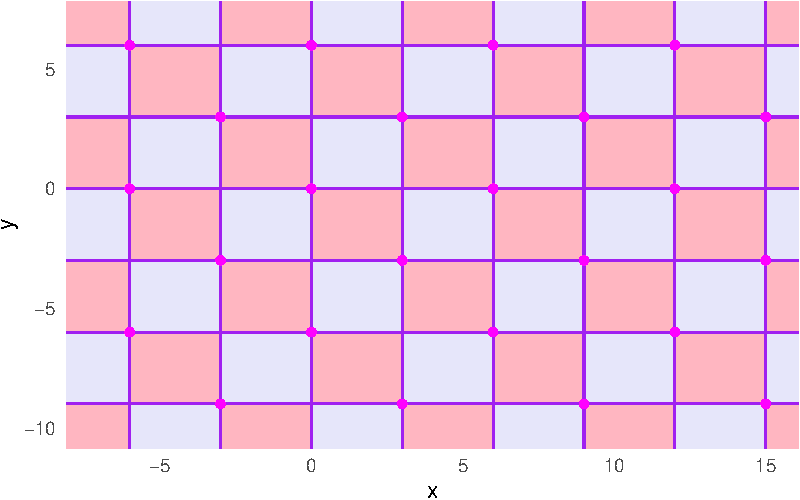
\includegraphics{handdrawn_files/figure-pdf/fourth-1.pdf}

}

\end{figure}

\hypertarget{fifth-tile}{%
\subsection*{Fifth Tile}\label{fifth-tile}}
\addcontentsline{toc}{subsection}{Fifth Tile}

\[
M = 
\begin{bmatrix} 12& 6\\ -3 & 1\end{bmatrix}
\]

\begin{Shaded}
\begin{Highlighting}[]
\FunctionTok{library}\NormalTok{(ggplot2)}
\DocumentationTok{\#\# original coordinates}
\NormalTok{A }\OtherTok{\textless{}{-}} \FunctionTok{matrix}\NormalTok{(}\FunctionTok{c}\NormalTok{(}\DecValTok{12}\NormalTok{, }\SpecialCharTok{{-}}\DecValTok{3}\NormalTok{), }\AttributeTok{ncol =} \DecValTok{1}\NormalTok{)}
\NormalTok{B }\OtherTok{\textless{}{-}} \FunctionTok{matrix}\NormalTok{(}\FunctionTok{c}\NormalTok{(}\DecValTok{6}\NormalTok{, }\DecValTok{1}\NormalTok{), }\AttributeTok{ncol =} \DecValTok{1}\NormalTok{)}

\DocumentationTok{\#\# coordinates for 4 copies/combos}
\NormalTok{copies }\OtherTok{\textless{}{-}} \SpecialCharTok{{-}}\DecValTok{10}\SpecialCharTok{:}\DecValTok{10}
\NormalTok{coefs }\OtherTok{\textless{}{-}} \FunctionTok{expand.grid}\NormalTok{(copies, copies)}

\NormalTok{x.coords }\OtherTok{\textless{}{-}}\NormalTok{ coefs}\SpecialCharTok{$}\NormalTok{Var1}\SpecialCharTok{*}\NormalTok{A[}\DecValTok{1}\NormalTok{] }\SpecialCharTok{+}\NormalTok{ coefs}\SpecialCharTok{$}\NormalTok{Var2}\SpecialCharTok{*}\NormalTok{B[}\DecValTok{1}\NormalTok{]}
\NormalTok{y.coords }\OtherTok{\textless{}{-}}\NormalTok{ coefs}\SpecialCharTok{$}\NormalTok{Var1}\SpecialCharTok{*}\NormalTok{A[}\DecValTok{2}\NormalTok{] }\SpecialCharTok{+}\NormalTok{ coefs}\SpecialCharTok{$}\NormalTok{Var2}\SpecialCharTok{*}\NormalTok{B[}\DecValTok{2}\NormalTok{]}

\NormalTok{plot.dat }\OtherTok{\textless{}{-}} \FunctionTok{data.frame}\NormalTok{(}\AttributeTok{x =}\NormalTok{ x.coords, }\AttributeTok{y =}\NormalTok{ y.coords)}
\NormalTok{p }\OtherTok{\textless{}{-}} \FunctionTok{ggplot}\NormalTok{(}\AttributeTok{data =}\NormalTok{ plot.dat, }\FunctionTok{aes}\NormalTok{(}\AttributeTok{x =}\NormalTok{ x, }\AttributeTok{y =}\NormalTok{ y)) }\SpecialCharTok{+}
    \FunctionTok{geom\_point}\NormalTok{() }\SpecialCharTok{+} 
    \FunctionTok{ylim}\NormalTok{(}\FunctionTok{c}\NormalTok{(}\SpecialCharTok{{-}}\DecValTok{14}\NormalTok{, }\DecValTok{7}\NormalTok{)) }\SpecialCharTok{+}
    \FunctionTok{xlim}\NormalTok{(}\FunctionTok{c}\NormalTok{(}\SpecialCharTok{{-}}\DecValTok{7}\NormalTok{, }\DecValTok{15}\NormalTok{)) }\SpecialCharTok{+} 
    \FunctionTok{geom\_rect}\NormalTok{(}\AttributeTok{xmin =} \SpecialCharTok{{-}}\DecValTok{7}\NormalTok{, }\AttributeTok{xmax =} \DecValTok{15}\NormalTok{, }\AttributeTok{ymin =} \SpecialCharTok{{-}}\DecValTok{14}\NormalTok{, }\AttributeTok{ymax =} \DecValTok{7}\NormalTok{, }
                        \AttributeTok{fill =} \StringTok{"\#FFFFFF00"}\NormalTok{, }\AttributeTok{col =} \StringTok{"black"}\NormalTok{) }\SpecialCharTok{+} 
    \FunctionTok{theme\_minimal}\NormalTok{()}


\DocumentationTok{\#\# could fix the grid to make these for printing!}

\DocumentationTok{\#\# create on{-}diag rectangles}
\NormalTok{p1 }\OtherTok{\textless{}{-}}\NormalTok{ p }\SpecialCharTok{+} \FunctionTok{geom\_rect}\NormalTok{(}\AttributeTok{xmin =}\NormalTok{ plot.dat}\SpecialCharTok{$}\NormalTok{x, }\AttributeTok{xmax =}\NormalTok{ plot.dat}\SpecialCharTok{$}\NormalTok{x }\SpecialCharTok{+}\NormalTok{ A[}\DecValTok{1}\NormalTok{], }
                            \AttributeTok{ymin =}\NormalTok{ plot.dat}\SpecialCharTok{$}\NormalTok{y, }\AttributeTok{ymax =}\NormalTok{ plot.dat}\SpecialCharTok{$}\NormalTok{y }\SpecialCharTok{{-}}\NormalTok{ B[}\DecValTok{2}\NormalTok{], }
                            \AttributeTok{fill =} \StringTok{"lightpink"}\NormalTok{, }\AttributeTok{col =} \StringTok{"darkred"}\NormalTok{) }\SpecialCharTok{+} 
    \FunctionTok{ylim}\NormalTok{(}\FunctionTok{c}\NormalTok{(}\SpecialCharTok{{-}}\DecValTok{10}\NormalTok{, }\DecValTok{7}\NormalTok{)) }\SpecialCharTok{+}
    \FunctionTok{xlim}\NormalTok{(}\FunctionTok{c}\NormalTok{(}\SpecialCharTok{{-}}\DecValTok{7}\NormalTok{, }\DecValTok{15}\NormalTok{)) }
\DocumentationTok{\#\# create off{-}diag rectangles}
\NormalTok{p2 }\OtherTok{\textless{}{-}}\NormalTok{ p1 }\SpecialCharTok{+} \FunctionTok{geom\_rect}\NormalTok{(}\AttributeTok{xmin =}\NormalTok{ plot.dat}\SpecialCharTok{$}\NormalTok{x, }\AttributeTok{xmax =}\NormalTok{ plot.dat}\SpecialCharTok{$}\NormalTok{x }\SpecialCharTok{+}\NormalTok{ B[}\DecValTok{1}\NormalTok{], }
                            \AttributeTok{ymin =}\NormalTok{ plot.dat}\SpecialCharTok{$}\NormalTok{y, }\AttributeTok{ymax =}\NormalTok{ plot.dat}\SpecialCharTok{$}\NormalTok{y }\SpecialCharTok{{-}}\NormalTok{ A[}\DecValTok{2}\NormalTok{], }
                            \AttributeTok{fill =} \StringTok{"\#E0FFFF"}\NormalTok{, }\AttributeTok{col =} \StringTok{"\#A2FFFF"}\NormalTok{)}
\NormalTok{p2 }\SpecialCharTok{+} \FunctionTok{geom\_point}\NormalTok{(}\AttributeTok{col =} \StringTok{"magenta"}\NormalTok{)}
\end{Highlighting}
\end{Shaded}

\begin{figure}[H]

{\centering 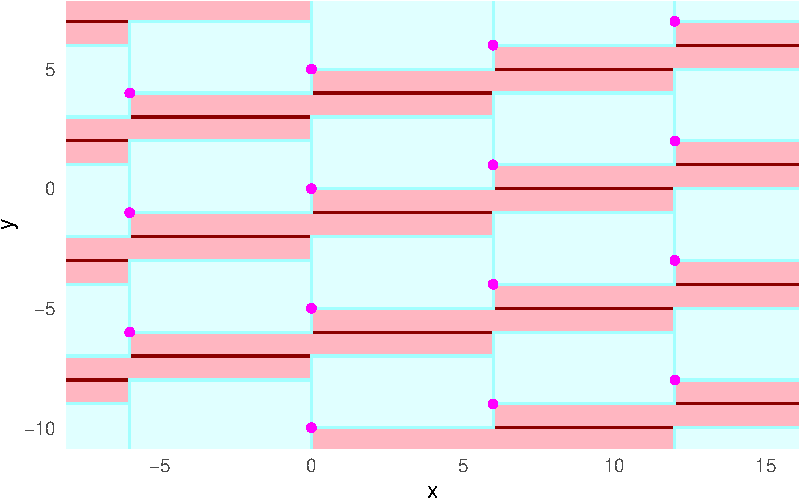
\includegraphics{handdrawn_files/figure-pdf/fifth-1.pdf}

}

\end{figure}

\hypertarget{sixth-tile}{%
\subsection*{Sixth tile}\label{sixth-tile}}
\addcontentsline{toc}{subsection}{Sixth tile}

\begin{Shaded}
\begin{Highlighting}[]
\FunctionTok{library}\NormalTok{(ggplot2)}
\DocumentationTok{\#\# original coordinates}
\NormalTok{A }\OtherTok{\textless{}{-}} \FunctionTok{matrix}\NormalTok{(}\FunctionTok{c}\NormalTok{(}\DecValTok{7}\NormalTok{, }\DecValTok{5}\NormalTok{), }\AttributeTok{ncol =} \DecValTok{1}\NormalTok{)}
\NormalTok{B }\OtherTok{\textless{}{-}} \FunctionTok{matrix}\NormalTok{(}\FunctionTok{c}\NormalTok{(}\DecValTok{6}\NormalTok{, }\DecValTok{2}\NormalTok{), }\AttributeTok{ncol =} \DecValTok{1}\NormalTok{)}

\DocumentationTok{\#\# coordinates for 4 copies/combos}
\NormalTok{copies }\OtherTok{\textless{}{-}} \SpecialCharTok{{-}}\DecValTok{15}\SpecialCharTok{:}\DecValTok{15}
\NormalTok{coefs }\OtherTok{\textless{}{-}} \FunctionTok{expand.grid}\NormalTok{(copies, copies)}

\NormalTok{x.coords }\OtherTok{\textless{}{-}}\NormalTok{ coefs}\SpecialCharTok{$}\NormalTok{Var1}\SpecialCharTok{*}\NormalTok{A[}\DecValTok{1}\NormalTok{] }\SpecialCharTok{+}\NormalTok{ coefs}\SpecialCharTok{$}\NormalTok{Var2}\SpecialCharTok{*}\NormalTok{B[}\DecValTok{1}\NormalTok{]}
\NormalTok{y.coords }\OtherTok{\textless{}{-}}\NormalTok{ coefs}\SpecialCharTok{$}\NormalTok{Var1}\SpecialCharTok{*}\NormalTok{A[}\DecValTok{2}\NormalTok{] }\SpecialCharTok{+}\NormalTok{ coefs}\SpecialCharTok{$}\NormalTok{Var2}\SpecialCharTok{*}\NormalTok{B[}\DecValTok{2}\NormalTok{]}

\NormalTok{plot.dat }\OtherTok{\textless{}{-}} \FunctionTok{data.frame}\NormalTok{(}\AttributeTok{x =}\NormalTok{ x.coords, }\AttributeTok{y =}\NormalTok{ y.coords)}
\NormalTok{p }\OtherTok{\textless{}{-}} \FunctionTok{ggplot}\NormalTok{(}\AttributeTok{data =}\NormalTok{ plot.dat, }\FunctionTok{aes}\NormalTok{(}\AttributeTok{x =}\NormalTok{ x, }\AttributeTok{y =}\NormalTok{ y)) }\SpecialCharTok{+}
    \FunctionTok{geom\_point}\NormalTok{() }\SpecialCharTok{+} 
    \FunctionTok{ylim}\NormalTok{(}\FunctionTok{c}\NormalTok{(}\SpecialCharTok{{-}}\DecValTok{14}\NormalTok{, }\DecValTok{7}\NormalTok{)) }\SpecialCharTok{+}
    \FunctionTok{xlim}\NormalTok{(}\FunctionTok{c}\NormalTok{(}\SpecialCharTok{{-}}\DecValTok{7}\NormalTok{, }\DecValTok{15}\NormalTok{)) }\SpecialCharTok{+} 
    \CommentTok{\# geom\_rect(xmin = {-}7, xmax = 15, ymin = {-}14, ymax = 7, }
    \CommentTok{\#                   fill = "\#FFFFFF00", col = "black") + }
    \FunctionTok{theme\_void}\NormalTok{()}


\DocumentationTok{\#\# could fix the grid to make these for printing!}

\DocumentationTok{\#\# create on{-}diag rectangles}
\NormalTok{p1 }\OtherTok{\textless{}{-}}\NormalTok{ p }\SpecialCharTok{+}\FunctionTok{geom\_rect}\NormalTok{(}\AttributeTok{xmin =}\NormalTok{ plot.dat}\SpecialCharTok{$}\NormalTok{x, }\AttributeTok{xmax =}\NormalTok{ plot.dat}\SpecialCharTok{$}\NormalTok{x }\SpecialCharTok{+}\NormalTok{ B[}\DecValTok{1}\NormalTok{], }
                            \AttributeTok{ymin =}\NormalTok{ plot.dat}\SpecialCharTok{$}\NormalTok{y, }\AttributeTok{ymax =}\NormalTok{ plot.dat}\SpecialCharTok{$}\NormalTok{y }\SpecialCharTok{{-}}\NormalTok{ A[}\DecValTok{2}\NormalTok{], }
                            \AttributeTok{fill =} \StringTok{"\#008b8b"}\NormalTok{, }\AttributeTok{alpha =}\NormalTok{ .}\DecValTok{1}\NormalTok{) }\SpecialCharTok{+} 
                            \FunctionTok{geom\_rect}\NormalTok{(}\AttributeTok{xmin =}\NormalTok{ plot.dat}\SpecialCharTok{$}\NormalTok{x, }\AttributeTok{xmax =}\NormalTok{ plot.dat}\SpecialCharTok{$}\NormalTok{x }\SpecialCharTok{+}\NormalTok{ B[}\DecValTok{1}\NormalTok{], }
                            \AttributeTok{ymin =}\NormalTok{ plot.dat}\SpecialCharTok{$}\NormalTok{y, }\AttributeTok{ymax =}\NormalTok{ plot.dat}\SpecialCharTok{$}\NormalTok{y }\SpecialCharTok{{-}}\NormalTok{ A[}\DecValTok{2}\NormalTok{], }
                            \AttributeTok{fill =} \StringTok{"\#FFFFFF00"}\NormalTok{, }\AttributeTok{col =} \StringTok{"grey"}\NormalTok{) }\SpecialCharTok{+}
                            \FunctionTok{geom\_rect}\NormalTok{(}\AttributeTok{xmin =}\NormalTok{ plot.dat}\SpecialCharTok{$}\NormalTok{x[}\DecValTok{481}\NormalTok{], }\AttributeTok{xmax =}\NormalTok{ plot.dat}\SpecialCharTok{$}\NormalTok{x[}\DecValTok{481}\NormalTok{] }\SpecialCharTok{+}\NormalTok{ B[}\DecValTok{1}\NormalTok{], }
                            \AttributeTok{ymin =}\NormalTok{ plot.dat}\SpecialCharTok{$}\NormalTok{y[}\DecValTok{481}\NormalTok{], }\AttributeTok{ymax =}\NormalTok{ plot.dat}\SpecialCharTok{$}\NormalTok{y[}\DecValTok{481}\NormalTok{] }\SpecialCharTok{{-}}\NormalTok{ A[}\DecValTok{2}\NormalTok{], }
                            \AttributeTok{fill =} \StringTok{"\#FFFFFF00"}\NormalTok{, }\AttributeTok{col =} \StringTok{"blue"}\NormalTok{) }\SpecialCharTok{+}
                            \FunctionTok{geom\_point}\NormalTok{(}\AttributeTok{col =} \StringTok{"magenta"}\NormalTok{) }\SpecialCharTok{+} 
                            \FunctionTok{ylim}\NormalTok{(}\FunctionTok{c}\NormalTok{(}\SpecialCharTok{{-}}\DecValTok{14}\NormalTok{, }\DecValTok{7}\NormalTok{)) }\SpecialCharTok{+}
                            \FunctionTok{xlim}\NormalTok{(}\FunctionTok{c}\NormalTok{(}\SpecialCharTok{{-}}\DecValTok{7}\NormalTok{, }\DecValTok{15}\NormalTok{))}




\FunctionTok{library}\NormalTok{(patchwork)}
\NormalTok{p2 }\OtherTok{\textless{}{-}}\NormalTok{ p }\SpecialCharTok{+} \FunctionTok{geom\_rect}\NormalTok{(}\AttributeTok{xmin =}\NormalTok{ plot.dat}\SpecialCharTok{$}\NormalTok{x, }\AttributeTok{xmax =}\NormalTok{ plot.dat}\SpecialCharTok{$}\NormalTok{x }\SpecialCharTok{+}\NormalTok{ A[}\DecValTok{1}\NormalTok{], }
                            \AttributeTok{ymin =}\NormalTok{ plot.dat}\SpecialCharTok{$}\NormalTok{y, }\AttributeTok{ymax =}\NormalTok{ plot.dat}\SpecialCharTok{$}\NormalTok{y }\SpecialCharTok{{-}}\NormalTok{ B[}\DecValTok{2}\NormalTok{], }
                            \AttributeTok{fill =} \StringTok{"yellow"}\NormalTok{, }\AttributeTok{alpha =}\NormalTok{ .}\DecValTok{3}\NormalTok{) }\SpecialCharTok{+}
                            \FunctionTok{geom\_rect}\NormalTok{(}\AttributeTok{xmin =}\NormalTok{ plot.dat}\SpecialCharTok{$}\NormalTok{x, }\AttributeTok{xmax =}\NormalTok{ plot.dat}\SpecialCharTok{$}\NormalTok{x }\SpecialCharTok{+}\NormalTok{ A[}\DecValTok{1}\NormalTok{], }
                            \AttributeTok{ymin =}\NormalTok{ plot.dat}\SpecialCharTok{$}\NormalTok{y, }\AttributeTok{ymax =}\NormalTok{ plot.dat}\SpecialCharTok{$}\NormalTok{y }\SpecialCharTok{{-}}\NormalTok{ B[}\DecValTok{2}\NormalTok{], }
                            \AttributeTok{fill =} \StringTok{"\#FFFFFF00"}\NormalTok{, }\AttributeTok{col =} \StringTok{"grey"}\NormalTok{) }\SpecialCharTok{+}
                            \FunctionTok{geom\_rect}\NormalTok{(}\AttributeTok{xmin =}\NormalTok{ plot.dat}\SpecialCharTok{$}\NormalTok{x[}\DecValTok{481}\NormalTok{], }\AttributeTok{xmax =}\NormalTok{ plot.dat}\SpecialCharTok{$}\NormalTok{x[}\DecValTok{481}\NormalTok{] }\SpecialCharTok{+}\NormalTok{ A[}\DecValTok{1}\NormalTok{], }
                            \AttributeTok{ymin =}\NormalTok{ plot.dat}\SpecialCharTok{$}\NormalTok{y[}\DecValTok{481}\NormalTok{], }\AttributeTok{ymax =}\NormalTok{ plot.dat}\SpecialCharTok{$}\NormalTok{y[}\DecValTok{481}\NormalTok{] }\SpecialCharTok{{-}}\NormalTok{ B[}\DecValTok{2}\NormalTok{], }
                            \AttributeTok{fill =} \StringTok{"\#FFFFFF00"}\NormalTok{, }\AttributeTok{col =} \StringTok{"orange"}\NormalTok{)}\SpecialCharTok{+}
                            \FunctionTok{geom\_point}\NormalTok{(}\AttributeTok{col =} \StringTok{"magenta"}\NormalTok{)}\SpecialCharTok{+} 
                            \FunctionTok{ylim}\NormalTok{(}\FunctionTok{c}\NormalTok{(}\SpecialCharTok{{-}}\DecValTok{14}\NormalTok{, }\DecValTok{7}\NormalTok{)) }\SpecialCharTok{+}
                            \FunctionTok{xlim}\NormalTok{(}\FunctionTok{c}\NormalTok{(}\SpecialCharTok{{-}}\DecValTok{7}\NormalTok{, }\DecValTok{15}\NormalTok{))}

\DocumentationTok{\#\# create off{-}diag rectangles}
\NormalTok{p\_both }\OtherTok{\textless{}{-}}\NormalTok{ p1 }\SpecialCharTok{+}  \FunctionTok{geom\_rect}\NormalTok{(}\AttributeTok{xmin =}\NormalTok{ plot.dat}\SpecialCharTok{$}\NormalTok{x, }\AttributeTok{xmax =}\NormalTok{ plot.dat}\SpecialCharTok{$}\NormalTok{x }\SpecialCharTok{+}\NormalTok{ A[}\DecValTok{1}\NormalTok{], }
                            \AttributeTok{ymin =}\NormalTok{ plot.dat}\SpecialCharTok{$}\NormalTok{y, }\AttributeTok{ymax =}\NormalTok{ plot.dat}\SpecialCharTok{$}\NormalTok{y }\SpecialCharTok{{-}}\NormalTok{ B[}\DecValTok{2}\NormalTok{], }
                            \AttributeTok{fill =} \StringTok{"yellow"}\NormalTok{, }\AttributeTok{alpha =}\NormalTok{ .}\DecValTok{2}\NormalTok{) }\SpecialCharTok{+}
                            \DocumentationTok{\#\# outlines}
                            \FunctionTok{geom\_rect}\NormalTok{(}\AttributeTok{xmin =}\NormalTok{ plot.dat}\SpecialCharTok{$}\NormalTok{x, }\AttributeTok{xmax =}\NormalTok{ plot.dat}\SpecialCharTok{$}\NormalTok{x }\SpecialCharTok{+}\NormalTok{ B[}\DecValTok{1}\NormalTok{], }
                            \AttributeTok{ymin =}\NormalTok{ plot.dat}\SpecialCharTok{$}\NormalTok{y, }\AttributeTok{ymax =}\NormalTok{ plot.dat}\SpecialCharTok{$}\NormalTok{y }\SpecialCharTok{{-}}\NormalTok{ A[}\DecValTok{2}\NormalTok{], }
                            \AttributeTok{fill =} \StringTok{"\#FFFFFF00"}\NormalTok{, }\AttributeTok{col =} \StringTok{"lightblue"}\NormalTok{, }\AttributeTok{lwd =} \DecValTok{2}\NormalTok{) }\SpecialCharTok{+}
                            \FunctionTok{geom\_rect}\NormalTok{(}\AttributeTok{xmin =}\NormalTok{ plot.dat}\SpecialCharTok{$}\NormalTok{x, }\AttributeTok{xmax =}\NormalTok{ plot.dat}\SpecialCharTok{$}\NormalTok{x }\SpecialCharTok{+}\NormalTok{ A[}\DecValTok{1}\NormalTok{], }
                            \AttributeTok{ymin =}\NormalTok{ plot.dat}\SpecialCharTok{$}\NormalTok{y, }\AttributeTok{ymax =}\NormalTok{ plot.dat}\SpecialCharTok{$}\NormalTok{y }\SpecialCharTok{{-}}\NormalTok{ B[}\DecValTok{2}\NormalTok{], }
                            \AttributeTok{fill =} \StringTok{"\#FFFFFF00"}\NormalTok{, }\AttributeTok{col =} \StringTok{"lightyellow"}\NormalTok{) }\SpecialCharTok{+} 
                            \FunctionTok{geom\_rect}\NormalTok{(}\AttributeTok{xmin =}\NormalTok{ plot.dat}\SpecialCharTok{$}\NormalTok{x[}\DecValTok{481}\NormalTok{], }\AttributeTok{xmax =}\NormalTok{ plot.dat}\SpecialCharTok{$}\NormalTok{x[}\DecValTok{481}\NormalTok{] }\SpecialCharTok{+}\NormalTok{ B[}\DecValTok{1}\NormalTok{], }
                            \AttributeTok{ymin =}\NormalTok{ plot.dat}\SpecialCharTok{$}\NormalTok{y[}\DecValTok{481}\NormalTok{], }\AttributeTok{ymax =}\NormalTok{ plot.dat}\SpecialCharTok{$}\NormalTok{y[}\DecValTok{481}\NormalTok{] }\SpecialCharTok{{-}}\NormalTok{ A[}\DecValTok{2}\NormalTok{], }
                            \AttributeTok{fill =} \StringTok{"\#FFFFFF00"}\NormalTok{, }\AttributeTok{col =} \StringTok{"blue"}\NormalTok{, }\AttributeTok{lwd =} \DecValTok{2}\NormalTok{) }\SpecialCharTok{+}
                            \FunctionTok{geom\_rect}\NormalTok{(}\AttributeTok{xmin =}\NormalTok{ plot.dat}\SpecialCharTok{$}\NormalTok{x[}\DecValTok{481}\NormalTok{], }\AttributeTok{xmax =}\NormalTok{ plot.dat}\SpecialCharTok{$}\NormalTok{x[}\DecValTok{481}\NormalTok{] }\SpecialCharTok{+}\NormalTok{ A[}\DecValTok{1}\NormalTok{], }
                            \AttributeTok{ymin =}\NormalTok{ plot.dat}\SpecialCharTok{$}\NormalTok{y[}\DecValTok{481}\NormalTok{], }\AttributeTok{ymax =}\NormalTok{ plot.dat}\SpecialCharTok{$}\NormalTok{y[}\DecValTok{481}\NormalTok{] }\SpecialCharTok{{-}}\NormalTok{ B[}\DecValTok{2}\NormalTok{], }
                            \AttributeTok{fill =} \StringTok{"\#FFFFFF00"}\NormalTok{, }\AttributeTok{col =} \StringTok{"yellow"}\NormalTok{) }\SpecialCharTok{+}
                            \FunctionTok{geom\_point}\NormalTok{(}\AttributeTok{col =} \StringTok{"magenta"}\NormalTok{) }\SpecialCharTok{+} 
                            \FunctionTok{ylim}\NormalTok{(}\FunctionTok{c}\NormalTok{(}\SpecialCharTok{{-}}\DecValTok{14}\NormalTok{, }\DecValTok{7}\NormalTok{)) }\SpecialCharTok{+}
                            \FunctionTok{xlim}\NormalTok{(}\FunctionTok{c}\NormalTok{(}\SpecialCharTok{{-}}\DecValTok{7}\NormalTok{, }\DecValTok{15}\NormalTok{))}
\DocumentationTok{\#\# add edges after}
\NormalTok{p1 }\SpecialCharTok{+}\NormalTok{ p2 }\SpecialCharTok{+}\NormalTok{ p\_both}
\end{Highlighting}
\end{Shaded}

\begin{figure}[H]

{\centering 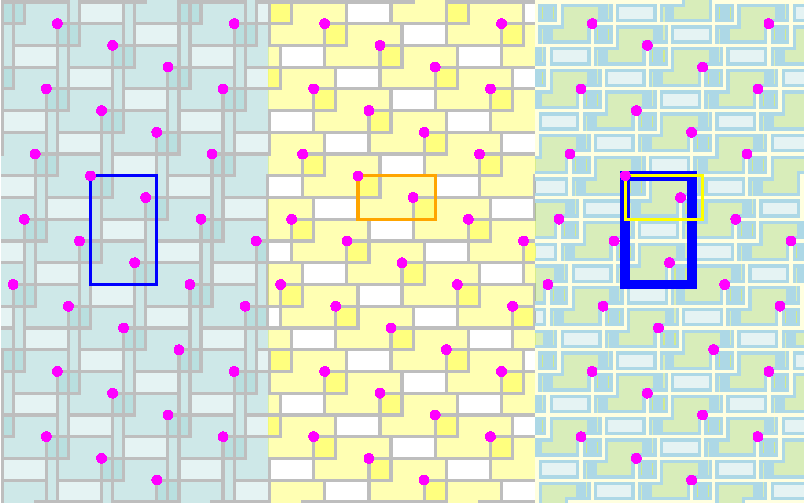
\includegraphics{handdrawn_files/figure-pdf/sixth-1.pdf}

}

\end{figure}

\bookmarksetup{startatroot}

\hypertarget{construction}{%
\chapter{Construction}\label{construction}}

\hypertarget{code-outline}{%
\section{Code outline}\label{code-outline}}

\textbf{Input:}

\begin{itemize}
\tightlist
\item
  A \((2+k) \times (2 +k)\) matrix \(M\)
\end{itemize}

\textbf{Step 1}

\begin{itemize}
\item
  calculate \(k\)
\item
  Create three new matrices:

  \begin{itemize}
  \item
    \(M_{TOP}\) is the \(2 \times (2+k)\) matrix consisting of the first
    two rows of \(M\)
  \item
    \(M_{BOT}\) is the \(k \times (2+k)\) matrix consisting of the
    remaining \(k\) rows of \(M\)
  \item
    \(M'\) is the \((2+k) \times (2 +k)\) matrix created by stacking
    \(M_{TOP}\) and \(-M_{BOT}\)
  \end{itemize}
\end{itemize}

\textbf{Step 2}

\begin{itemize}
\item
  For each \(\sigma \in \binom{[2+k]}{2}\), define \(S_{\sigma}(M)\) as
  follows:

  \begin{tcolorbox}[enhanced jigsaw, titlerule=0mm, arc=.35mm, coltitle=black, left=2mm, colframe=quarto-callout-note-color-frame, opacitybacktitle=0.6, bottomrule=.15mm, rightrule=.15mm, breakable, leftrule=.75mm, title=\textcolor{quarto-callout-note-color}{\faInfo}\hspace{0.5em}{Notation: \(\binom{[n]}{k}\)}, bottomtitle=1mm, toptitle=1mm, toprule=.15mm, colback=white, opacityback=0, colbacktitle=quarto-callout-note-color!10!white]

  The notation is shorthand for the set of all subsets of
  \(\{1, 2, \dots, n\}\) of size \(k\).

  For example, if \(n = 3\) and \(k=2\),
  \[\binom{[n]}{k} =  \binom{[3]}{2} = FIXME\]

  \end{tcolorbox}

  \begin{itemize}
  \item
    Start with \(M'\),

    \begin{itemize}
    \tightlist
    \item
      Consider \(i^{th}\) column for \(i \in \{1, 2, \dots, k+2\}\). If
      :

      \begin{itemize}
      \tightlist
      \item
        \(i \in \sigma\): zero out bottom \(k\) entries
      \item
        \(i \not\in \sigma\): zero out the top 2 entries
      \end{itemize}
    \end{itemize}
  \end{itemize}
\end{itemize}

\begin{figure}

{\centering 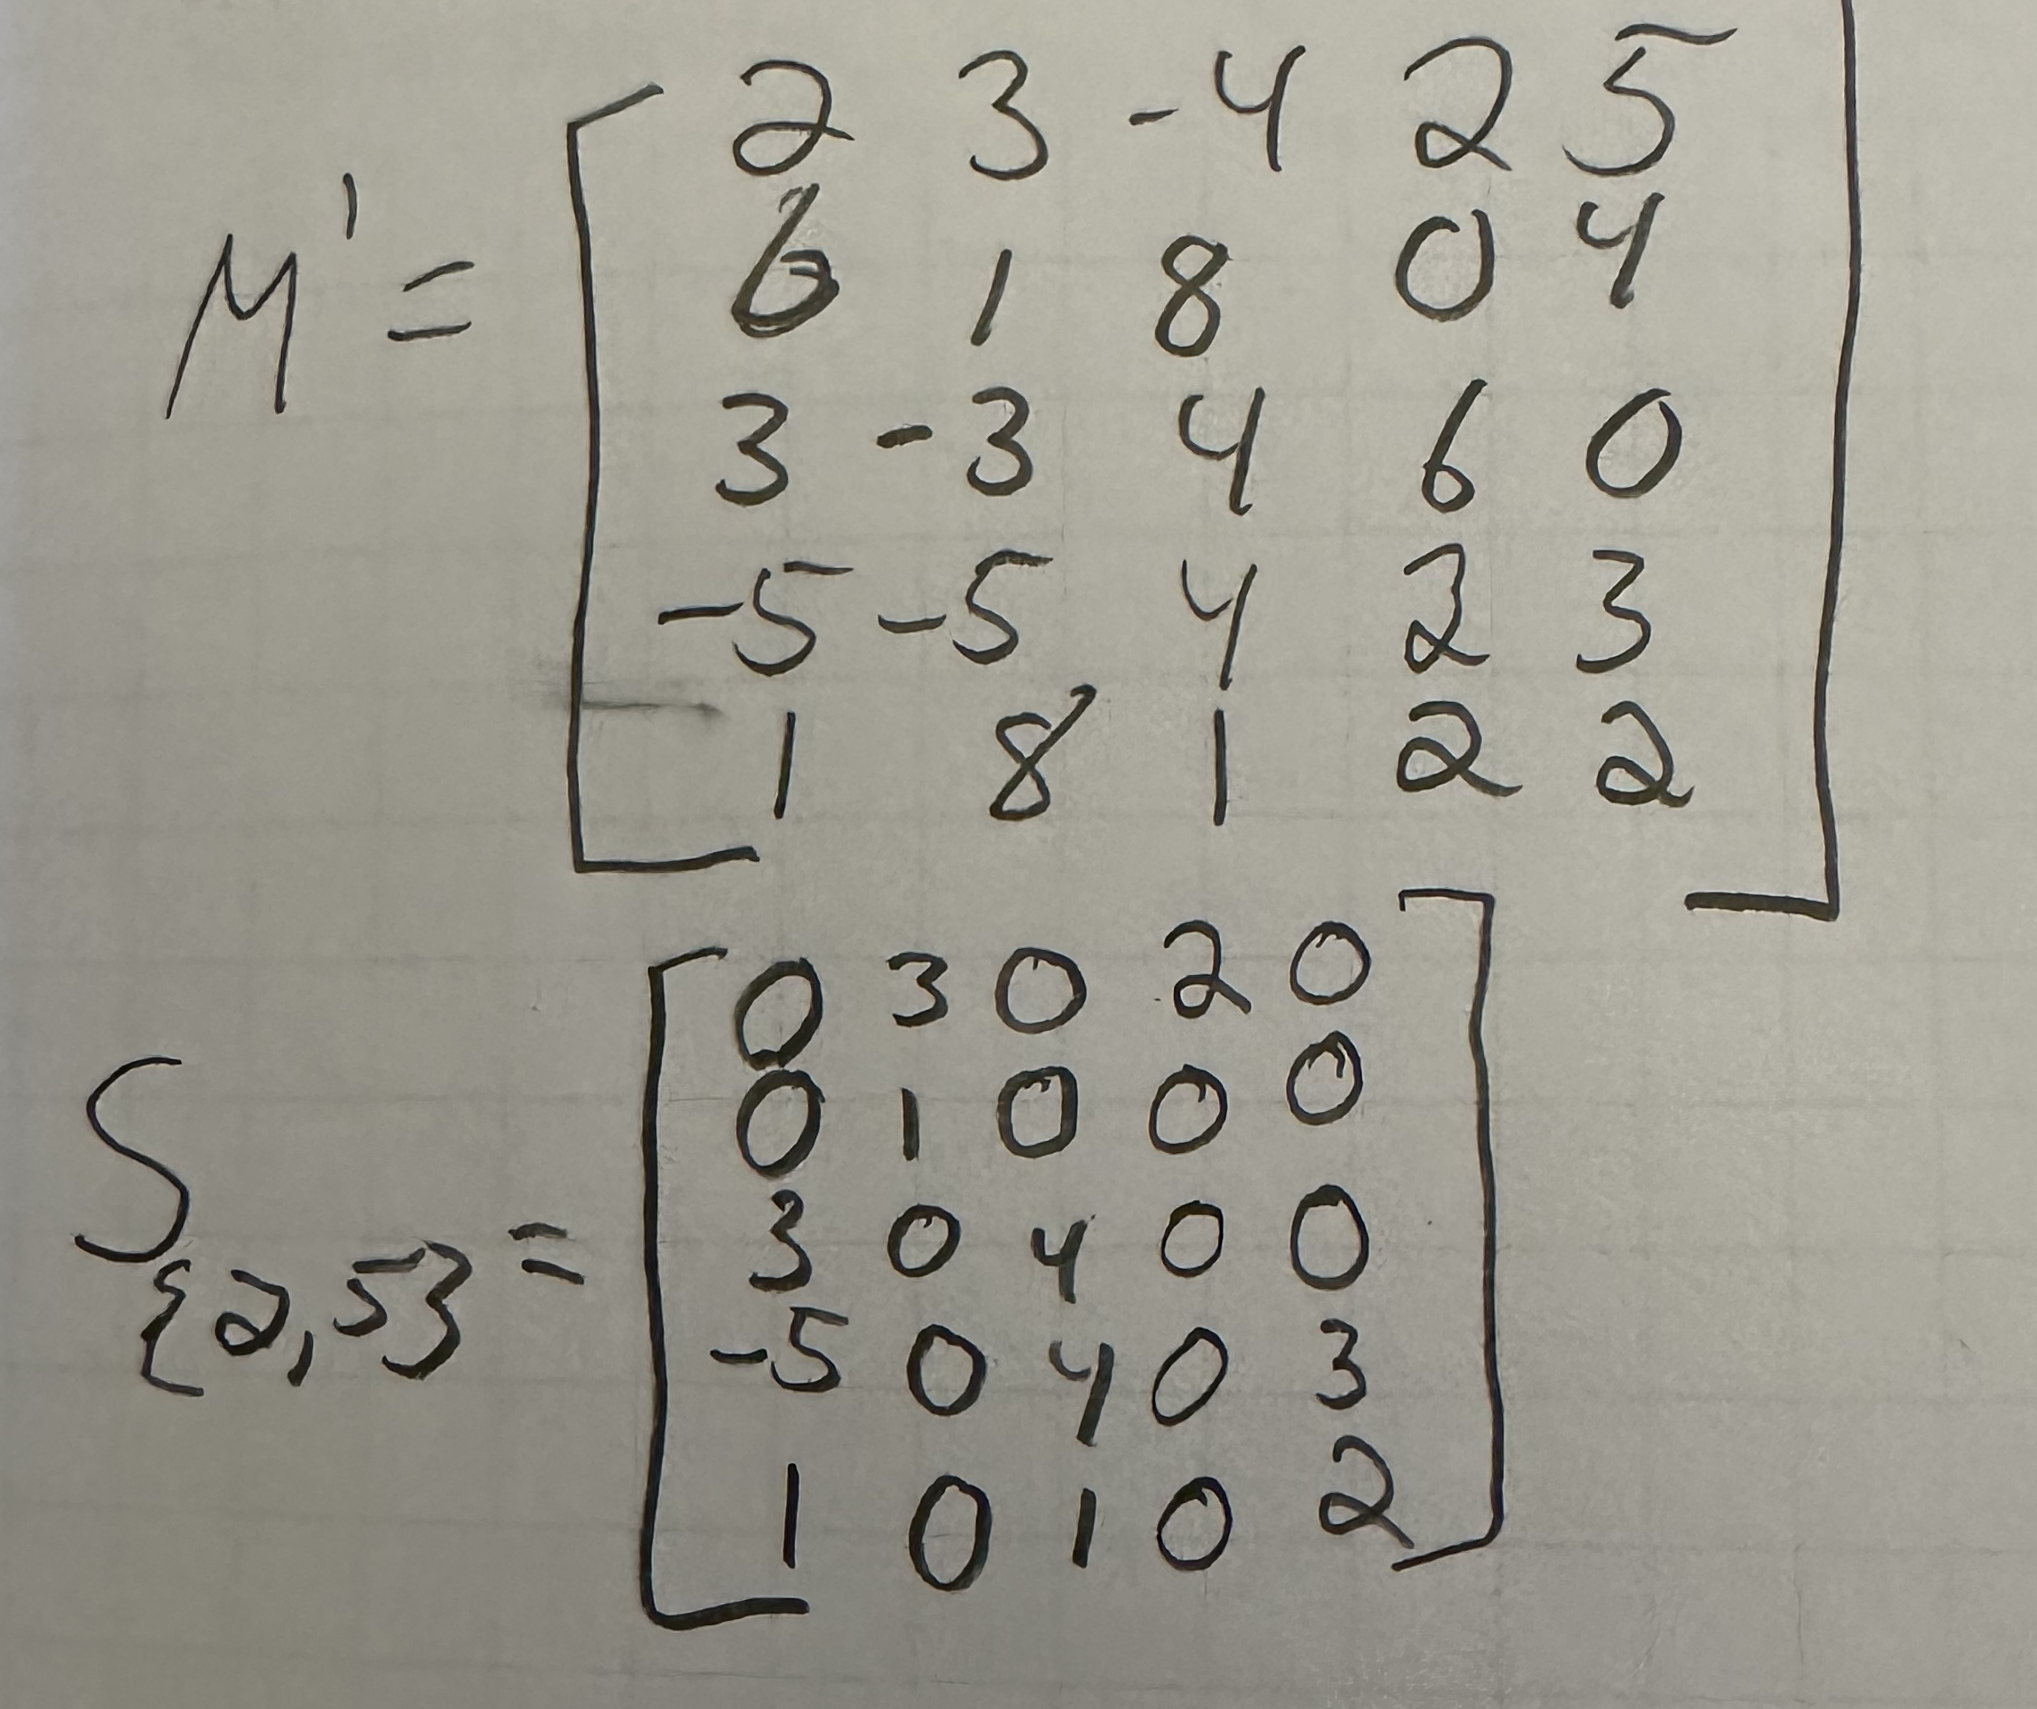
\includegraphics{images/matrix_example.png}

}

\caption{Here, \(k = 3\) and \(\sigma = \{2, 5\}\).}

\end{figure}

\begin{itemize}
\tightlist
\item
  After this process, you will end up with
  \(\frac{1}{2}k^2 + \frac{3}{2}k + 1\) matrices
\end{itemize}

\textbf{Step 3}

Consider the matrices \(\{S_\sigma\}\). Each of these matrices
corresponds to a \(2+k\)-dimensional shape (the
\href{https://en.wikipedia.org/wiki/Parallelepiped\#:~:text=In\%20geometry\%2C\%20a\%20parallelepiped\%20is,cube\%20relates\%20to\%20a\%20square.}{fundamental
parallelepiped} \(\Pi \left ( S_\sigma\right )\) defined by the columns
of that matrix).

\begin{tcolorbox}[enhanced jigsaw, titlerule=0mm, arc=.35mm, coltitle=black, left=2mm, colframe=quarto-callout-note-color-frame, opacitybacktitle=0.6, bottomrule=.15mm, rightrule=.15mm, breakable, leftrule=.75mm, title=\textcolor{quarto-callout-note-color}{\faInfo}\hspace{0.5em}{The fundamental parallelepiped \(\Pi(S_\sigma)\)}, bottomtitle=1mm, toptitle=1mm, toprule=.15mm, colback=white, opacityback=0, colbacktitle=quarto-callout-note-color!10!white]

Note that

\[\Pi \left ( S_\sigma\right ) = \{S_\sigma \cdot (x_1, \dots, x_{k+2})'\}\]
Think of the \(x_i\) as representing the interval \([0,1]\), so that you
are getting a shape. In other words, \(\Pi\) is the
\href{https://en.wikipedia.org/wiki/Minkowski_addition}{Minkowski sum}
of the columns of \(S_\sigma\).

\end{tcolorbox}

For each \(\sigma\), want to visualize a collection of parallelepipeds,
\(\Pi \left ( S_\sigma\right ) + Mz\), where \(z \in \mathbb{Z}^{k+2}\).
(FIXME: in practice we won't want to generate individual plots because
there will be too many, we just want to emphasize a given \(S_\sigma\)
in the plots discussed next.)

The desired end product is to create two visualizations: one of all
positive \(S_\sigma\) and one of all negative \(S_\sigma\).

\begin{tcolorbox}[enhanced jigsaw, titlerule=0mm, arc=.35mm, coltitle=black, left=2mm, colframe=quarto-callout-note-color-frame, opacitybacktitle=0.6, bottomrule=.15mm, rightrule=.15mm, breakable, leftrule=.75mm, title=\textcolor{quarto-callout-note-color}{\faInfo}\hspace{0.5em}{What about \(det(S_\sigma) = 0\)?}, bottomtitle=1mm, toptitle=1mm, toprule=.15mm, colback=white, opacityback=0, colbacktitle=quarto-callout-note-color!10!white]

The determinant measures volume. So, in this case, the volume of the
parallelepiped is 0, so there is nothing to visualize.

\end{tcolorbox}

Also, that parallelepiped is more than 3D so there will need to be a
choice made in which slices to take for visualization.



\end{document}
